\section{Moti Longitudinali}

Il controllo dei moti longitudinali ha quindi un duplice obiettivo: stabilizzare il sistema, che in catena aperta non risulta essere BIBO stabile, e implementare un autopilota per il mantenimento dell'altitudine.

Poiché non si tratta di un sistema SAS (\textit{Stability Augmentation System}), non è necessario progettare il controllore tenendo conto la risposta del velivolo ai comandi del pilota.
È invece sufficiente garantire una dinamica stabile e confortevole per piloti e passeggeri. A tale scopo, si ricerca un controllore che assicuri uno smorzamento $\zeta \approx 0.5$ e una pulsazione naturale $\omega_n \gg 1$ rad/s.

\subsection{Architettura}

L'analisi del luogo delle radici della funzione di trasferimento $W_{\delta_e \rightarrow z}$ mostra chiaramente che un semplice controllore proporzionale non è in grado di garantire le prestazioni richieste, in quanto presenta sempre poli a parte reale positiva per qualunque valore di guadagno $k$.

Come è prassi comune in ambito aeronautico, il controllo dei moti longitudinali viene affrontato in due fasi distinte:
\begin{sitemize}
    \item \textbf{Stabilizzazione del sistema}: in particolare si interviene sul modo \textit{short-period} (\ref{subsubsec:short_period}) mediante un controllo retroazionato della velocità angolare $q$ e dell'angolo di beccheggio $\theta$;
    \item \textbf{Navigazione}: una volta stabilizzato il sistema, si implementa un controllo dell'altitudine, utilizzando un controllore sulla quota $z$.
\end{sitemize}

\begin{figure}[H]
    \centering
    \begin{tikzpicture}
        \node[draw,
            circle,
            minimum size=0.5cm,
        ] (sum_outer) at (0,0){};

        % Controller
        \node [draw,
            minimum width=2.4cm,
            minimum height=1.2cm,
            right=1.5cm of sum_outer
        ]  (controller) {$C(s)$};

        \node[draw,
            circle,
            minimum size=0.5cm,
            right=1.5cm of controller
        ] (sum_inner) {};

        % System
        \node [draw,
            minimum width=2.4cm,
            minimum height=2.8cm,
            right=1.5cm of sum_inner,
            yshift=0.8cm
        ]  (system) {$Sistema$};

        % Sensor block
        \node [draw,
            minimum width=1.5cm,
            minimum height=1cm,
            below right= 1cm and 1.5cm of sum_inner
        ]  (k_q) {$k_q$};

        % Sensor block
        \node [draw,
            minimum width=1.5cm,
            minimum height=1cm,
            below right= 2.5cm and 1.5cm of sum_inner
        ]  (k_theta) {$k_{\theta}$};


        \draw[-stealth] (system.330) -- ++ (1.25,0)
        node[midway](output_q){}node[midway,above]{$q(t)$};
        \draw[-stealth] (system.0) -- ++ (2,0)
        node[midway](output_theta){}node[midway,above]{$\theta(t)$};
        \draw[-stealth] (system.30) -- ++ (2.75,0)
        node[midway, above](output_z){}node[midway,above]{$z(t)$};

        \draw[stealth-] (system.150) -- ++ (-1.5,0)
        node[midway,above]{$\delta_t(t)$};

        \draw[-stealth] (controller.east) -- ++ (1.5,0)
        node[midway,above]{$u(t)$};

        \draw[-stealth] (sum_inner.east) -- ++ (1.5,0)
        node[midway,above]{$\delta_e(t)$};

        \draw[-stealth] (sum_outer.east) -- ++ (1.5,0)
        node[midway,above]{$e_{z}(t)$};
        \draw[stealth-] (sum_outer.west) -- ++ (-1.25,0)
        node[midway,above]{$\hat{z}(t)$};

        \draw[-stealth] (k_q.west) -| (sum_inner.310);
        \draw[-stealth] (output_q.center) |- (k_q.east);

        \draw[-stealth] (k_theta.west) -| (sum_inner.240);
        \draw[-stealth] (output_theta.center) |- (k_theta.east);

        \draw [-stealth] (output_z) |- (0,-4) -| (sum_outer);

        \node at ($(sum_outer)+(-0.25,0.40)$) {$+$};
        \node at ($(sum_outer)+(-0.25,-0.4)$) {$-$};

        \node at ($(sum_inner)+(-0.25,0.4)$) {$+$};
        \node at ($(sum_inner)+(-0.30,-0.4)$) {$-$};
        \node at ($(sum_inner)+(0.30,-0.4)$) {$-$};
    \end{tikzpicture}
\end{figure}

\subsection{Analisi dei Parametri}

\subsubsection{Loop Interno}

Al fine di stabilizzare il sistema, è necessario impiegare entrambi i segnali $q$ e $\theta$ come variabili di retroazione, come risulterà evidente dall'analisi dei rispettivi luoghi delle radici.
\\[10pt]
Il luogo delle radici rispetto alla funzione di trasferimento $W_{\delta_e \rightarrow q}$ mostra che il guadagno minimo necessario per stabilizzare i poli associati al modo \textit{phugoid} è circa $k \approx -5.02$. Tuttavia, per questo valore, i due poli associati al modo \textit{short-period} risultano reali, hanno quindi coefficiente di smorzamento $\zeta = 1$, che non soddisfa i requisiti richiesti dal problema.

\begin{figure}[H]
    \centering
    \begin{minipage}{.48\textwidth}
        \centering
        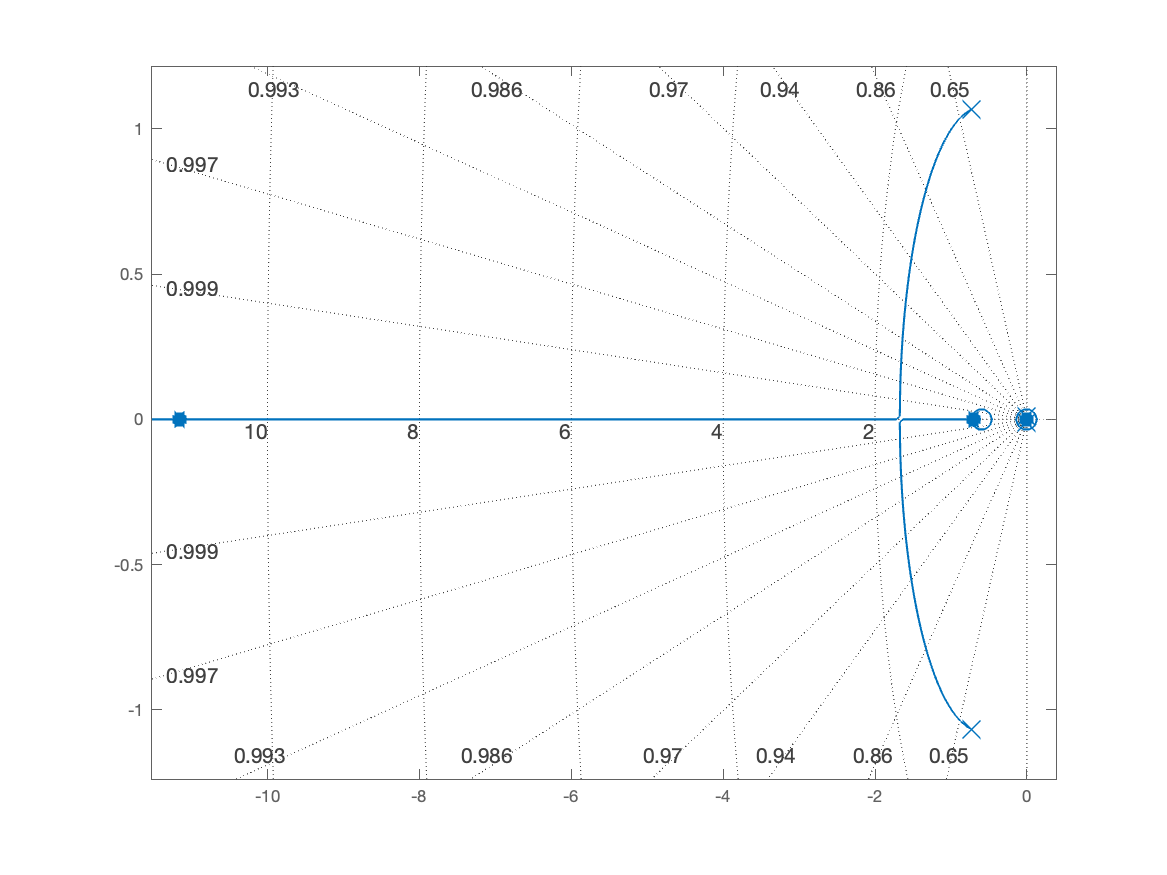
\includegraphics[width=1\linewidth]{Immagini/root_q_only_1.pdf}
        \captionof{figure}{\texttt{rlocus} di $W_{\delta_e \rightarrow q}$ con evidenziati i risultati per $k = -5.02$}
    \end{minipage}
    \hspace{0.02\textwidth}
    \begin{minipage}{.48\textwidth}
        \centering
        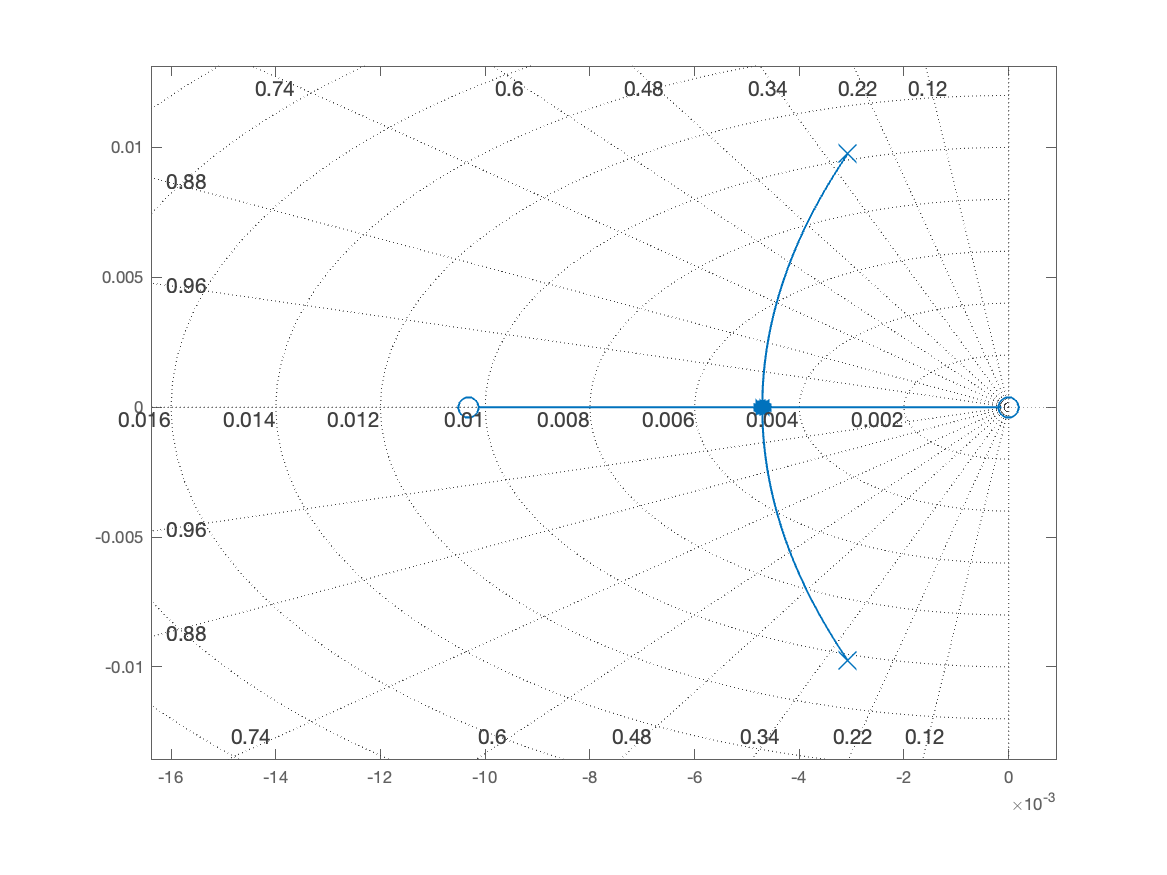
\includegraphics[width=1\linewidth]{Immagini/root_q_only_2.pdf}
        \captionof{figure}{Dettaglio che mostra i poli associati al modo \textit{phugoid}}
    \end{minipage}
\end{figure}

Analogamente, anche nel caso della sola retroazione su $\theta$, non è possibile soddisfare le specifiche del progetto. Il guadagno minimo per stabilizzare i poli associati al modo \textit{phugoid} è circa $k \approx -0.05337$, ma i poli del modo \textit{short-period} in questo caso hanno una frequenza naturale pari a $\omega_n = 1.33 \text{ rad/s}$, superiore al valore desiderabile.
\begin{figure}[H]
    \centering
    \begin{minipage}{.48\textwidth}
        \centering
        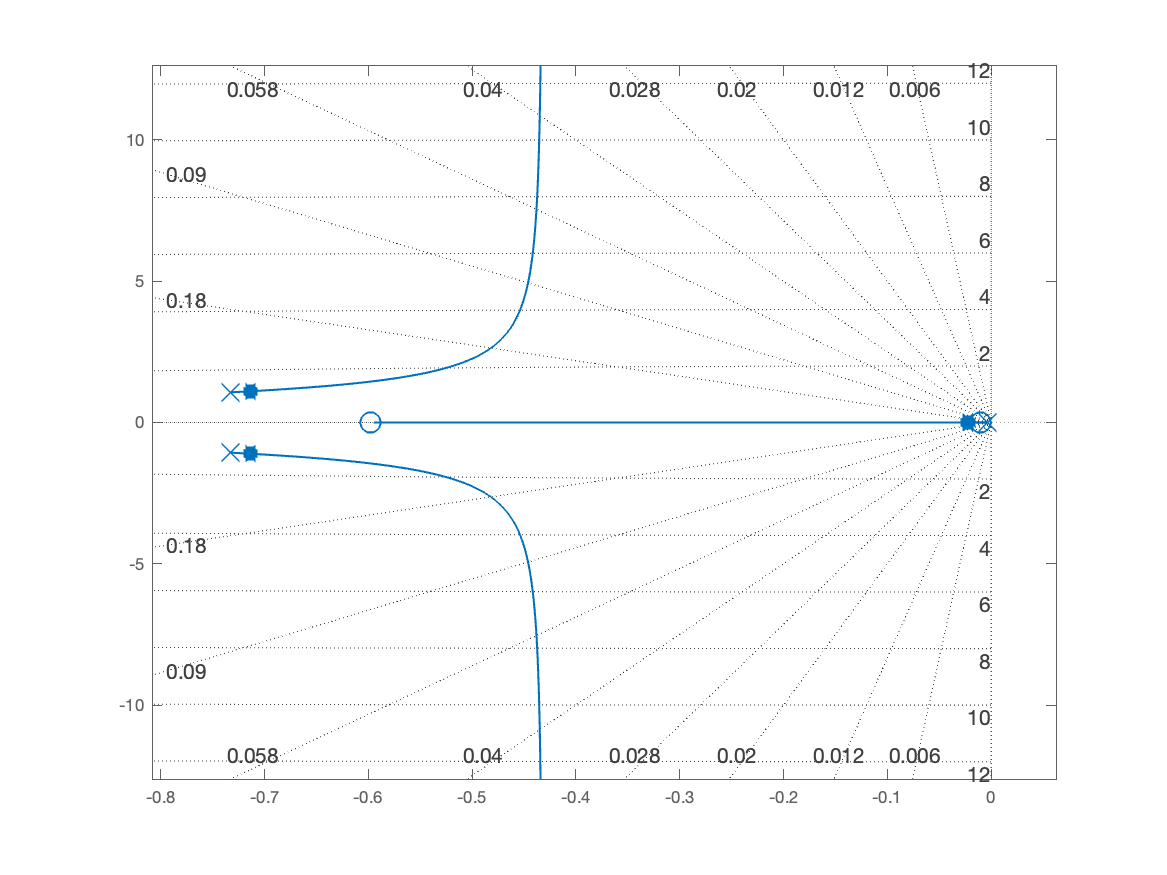
\includegraphics[width=1\linewidth]{Immagini/root_theta_only_1.pdf}
        \captionof{figure}{\texttt{rlocus} di $W_{\delta_e \rightarrow \theta}$ con evidenziati i risultati per $k = -0.05337$}
    \end{minipage}
    \hspace{0.02\textwidth}
    \begin{minipage}{.48\textwidth}
        \centering
        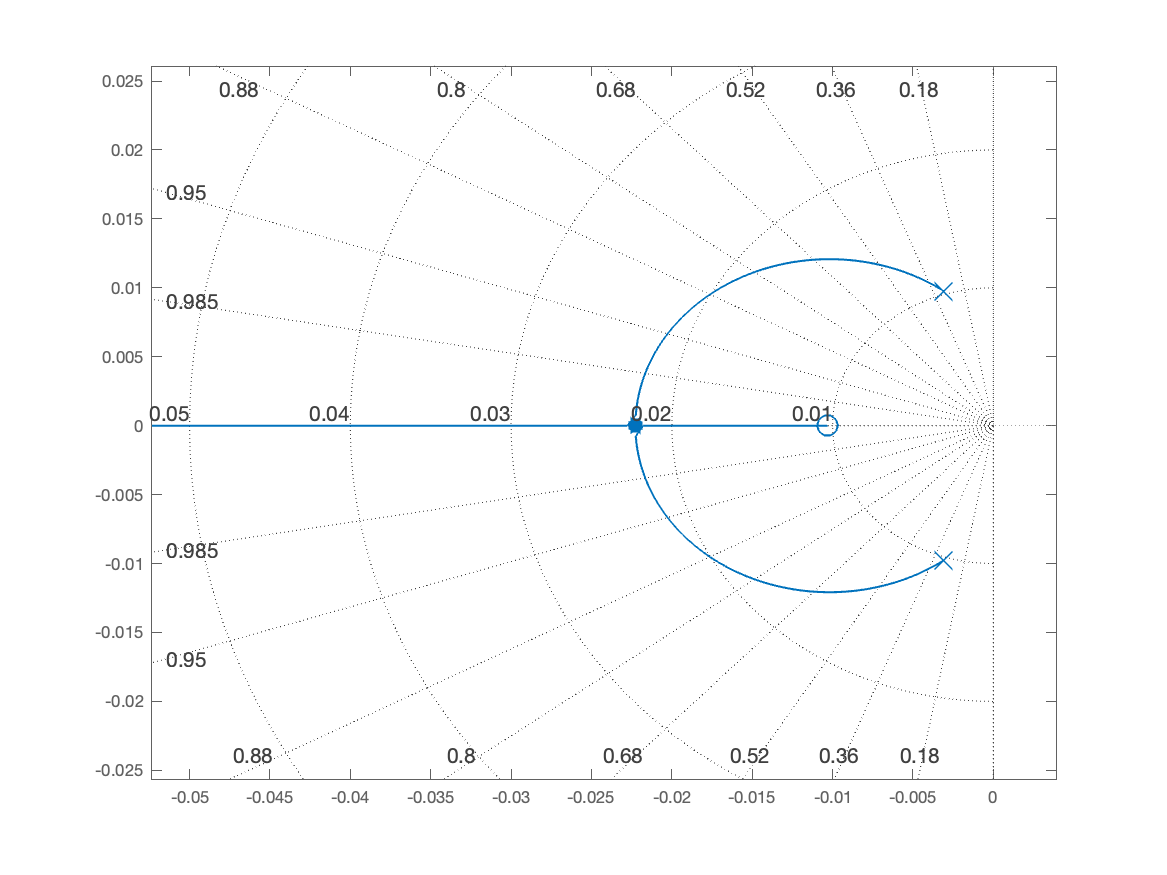
\includegraphics[width=1\linewidth]{Immagini/root_theta_only_2.pdf}
        \captionof{figure}{Dettaglio che mostra i poli associati al modo \textit{phugoid}}
    \end{minipage}
\end{figure}

È possibile ottenere una soluzione con caratteristiche migliori utilizzando entrambi i guadagni, in particolare vengono scelti $k_q = -1.73$ e $k_{\theta} = -6.10$.

Con tali valori, i poli del sistema si trovano in $s = 0, -0.0104, -0.539, -2.25 \pm j2.99$. I due poli complessi associati al modo \textit{short-period} hanno coefficiente di smorzamento $\zeta = 0.602$ e pulsazione naturale $\omega_n = 3.75 rad/s$, valori che rispettano le specifiche del problema.

\subsubsection{Loop Esterno}

Il loop esterno ha il compito di spostare il polo in $s = 0$, fornendo al contempo le prestazioni desiderate. A tal fine, viene adottato un controllore PD:
\begin{equation*}
    C(s) = -0.0082844 (0.1 + s)
\end{equation*}

I parametri del controllore (guadagno e posizione del polo reale) sono stati determinati mediante la funzionalità di \textit{optimization-based tuning} fornita dal tool \texttt{Control System Designer}.

Si nota che i valori trovati dal modello di ottimizzazione sono tali perché rappresentano un compromesso tra i tempi di risposta e smorzamento:
un incremento di $\left|k\right|$ farebbe scendere il coefficiente di smorzamento dei poli associati al modo \textit{short-period} al di sotto di $0.5$,
mentre una riduzione $\left|k\right|$ porterebbe ad una dinamica più lenta, poiché due poli si avvicinerebbero all'origine.

\begin{figure}[H]
    \centering
    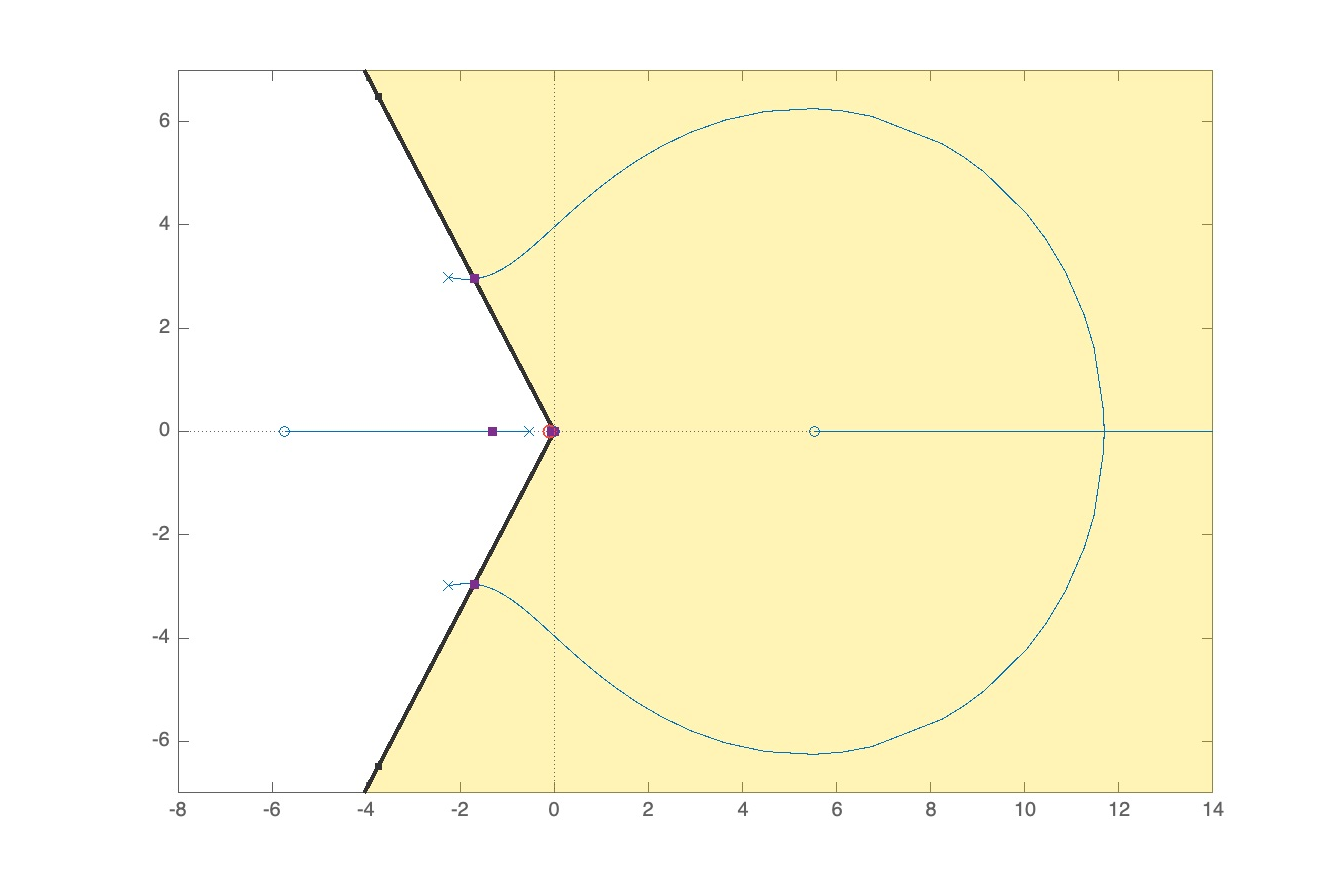
\includegraphics[width=0.6\linewidth]{Immagini/root_h.pdf}
    \caption{Luogo delle radici per $C(s) = k(z_0 + s)$, $k < 0$}
\end{figure}

\begin{figure}[H]
    \centering
    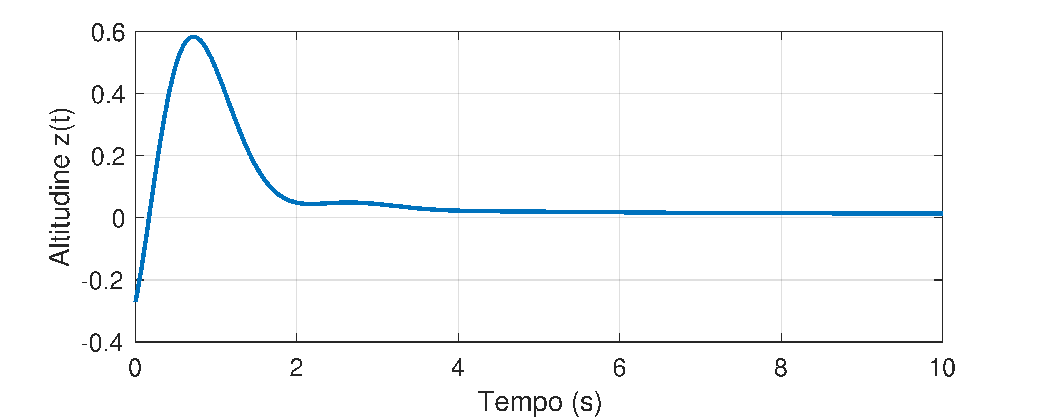
\includegraphics[width=0.7\linewidth]{Immagini/impulse_longitudinal.pdf}
    \caption{Risposta impulsiva del sistema}
\end{figure}

\subsection{Prestazioni}

Per il sistema controllato dai controllori ottenuti precedentemente, si ricavano i seguenti parametri:
\begin{sitemize}
    \item coefficiente di smorzamento associato al modo \textit{short-period}: $\zeta = 0.5$
    \item frequenza naturale associata al modo \textit{short-period}: $\omega_{n} = 3.41\, rad/s$
    \item tempo di salita, ovvero tempo necessario per arrivare al $90\%$ del valore di regime ($y(\infty)$): $T_{s} = 34.11\, s$
    \item sovraelongazione percentuale: $S_{\%} = \frac{y_{max}}{y(\infty)} -1 = 0\%$
    \item sottoelongazione percentuale: $U_{\%} = \frac{y_{min}}{y(\infty)} -1 = 2.42\%$
    \item tempo di assestamento, ovvero il tempo necessario perché la risposta entri nella fascia di valori compresi tra $\pm2\%\cdot y(\infty)$ senza più uscirne: $T_{a} = 238.28\, s$
\end{sitemize}

\begin{figure}[H]
    \centering
    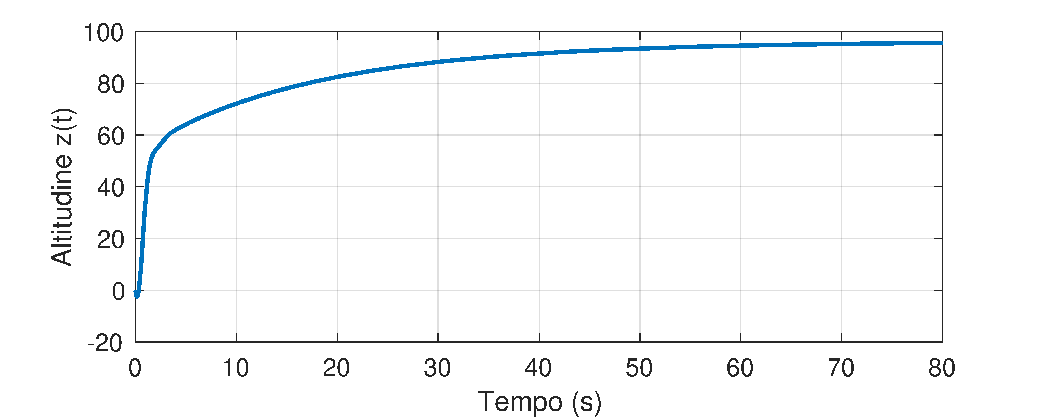
\includegraphics[width=0.7\linewidth]{Immagini/step_longitudinal.pdf}
    \caption{Risposta del sistema al gradino di 100 ft}
\end{figure}

Il sistema di controllo sviluppato consente di soddisfare i requisiti specificati dal problema, stabilizzando la dinamica del velivolo e mantenendo correttamente una determinata altitudine.
